\documentclass[12pt,oneside,letterpaper]{article}
\usepackage[margin=1in]{geometry}
\usepackage{listings}
\usepackage{graphicx}
\usepackage{hyperref}
\usepackage{amsmath}
\title{OpenGM Demo}
\author{Vikas Dhiman}
\begin{document}
\maketitle
\section{Installation}
Please follow \href{http://www.andres.sc/publications/opengm-2.0.2-beta-manual.pdf}{OpenGM manual} for installation.

If you are facing problems OpenGM installation, we have a virtual machine setup
which I'll post on piazza. 

\section{Introduction}
Using probablistic graphical models consists of two main steps. 
\begin{enumerate}
  \item Modeling
  \item Inference
\end{enumerate}

However, when we are using a standard library like OpenGM, we have few more steps that need to be considered.
\begin{enumerate}
  \item Modeling
  \begin{enumerate}
    \item Adapting the model to OpenGM compatible format
    \item Coding the model
  \end{enumerate}
  \item Inference
    \begin{enumerate}
      \item Identifying the problem to OpenGM compatible format
      \item Coding and running the model
      \item Mapping back the solution from OpenGM to our original problem
    \end{enumerate}
\end{enumerate}

OpenGM is vast library with plethora of features. We can't cover all features
in today's demo, but hopefully this demo will give you a headstart with the
library. The official manual starts with abstract definitions followed by
examples. We will try the opposite methodology, starting with example and then
generalizing (abstraction). This will enable students to have a choice, between two methodologies.

\section{Example}
\subsection{Modeling}
Modeling is defining the relationships and assumptions between various elements
of the problem in a mathematical framework. For this example, we assume that
the graphical model is given as a Bayes network.  We will consider the Bayesian
network provided in Figure 3.4 (Page 53) from the text book.

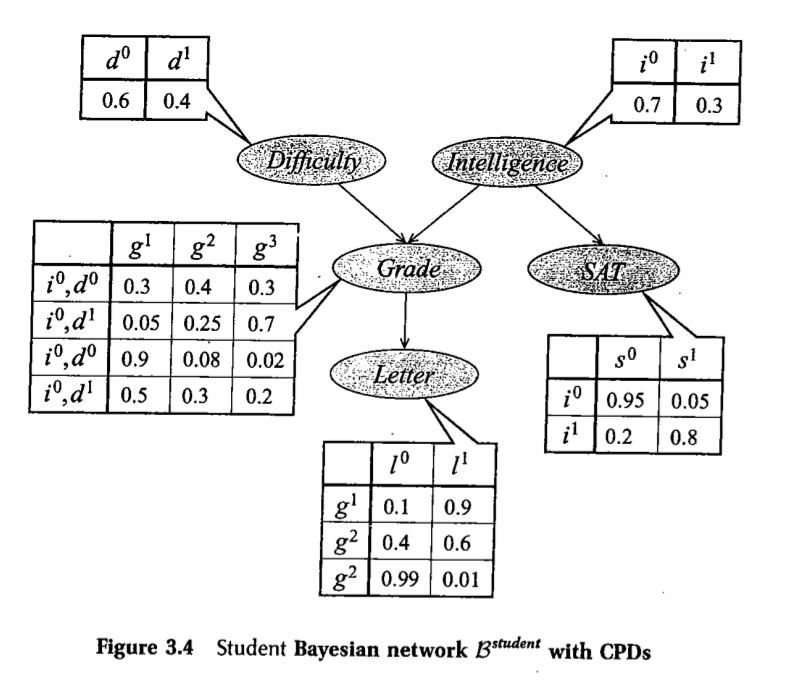
\includegraphics[width=\textwidth]{media/examplebayesnet.png}

\subsection{Adapting the model}
We note that the above Bayesian model represents explicit factorization of
joint probability distribution of all the random variables.
\begin{align}
  P(I, D, G, S, L) &= P_I(I)P_D(D)P_{G|I,D}(G|I, D)P_{S|I}(S|I)P_{L|G}(L|G)
\end{align}
where each factor corresponds to a function that is defined in Figure 3.4.

Note that each function depends only on a subset of random variables, for
example, $P_I(.)$ only depends on $I$, and $P_{G|I,D}(.)$ depends only on
$G$,$I$ and $D$.

Such a factorization can be represented as something called a \emph{factor graph} (Fig~\ref{fig:fg2}).
\begin{figure}
  \centering
  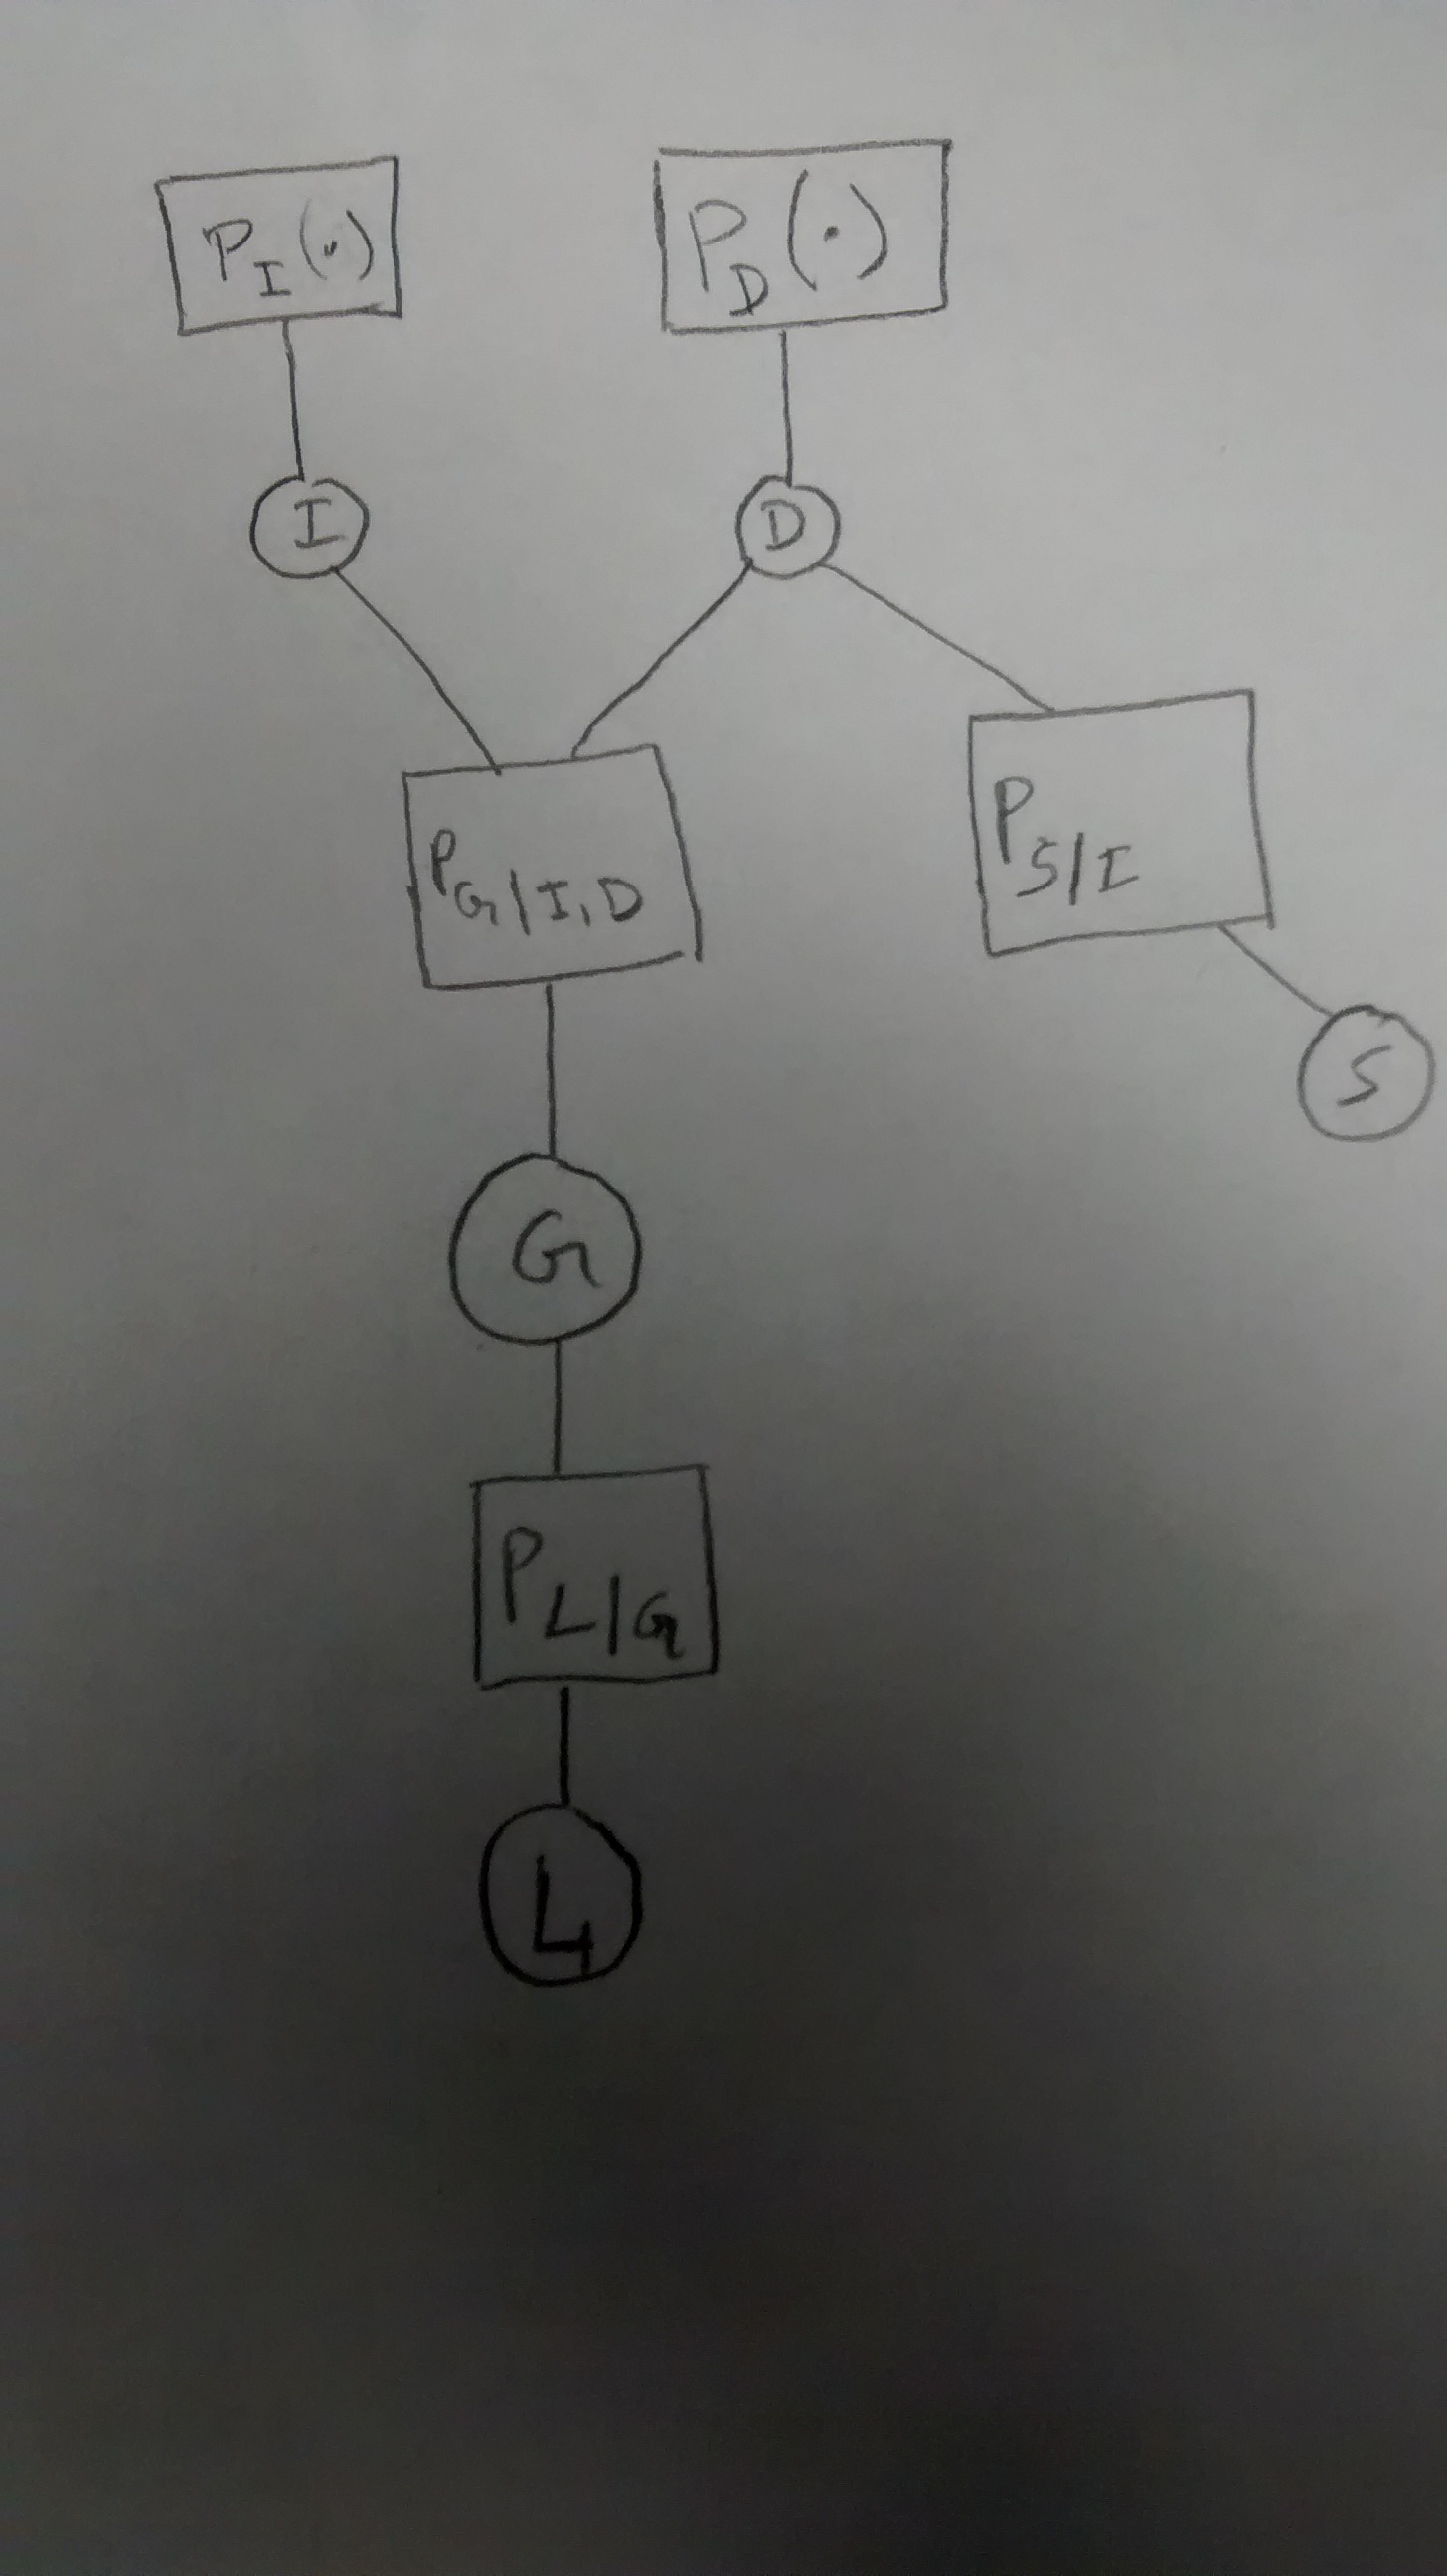
\includegraphics[height=0.58\textwidth, trim=0 8in 0 0, clip]{media/fg1.jpg}
  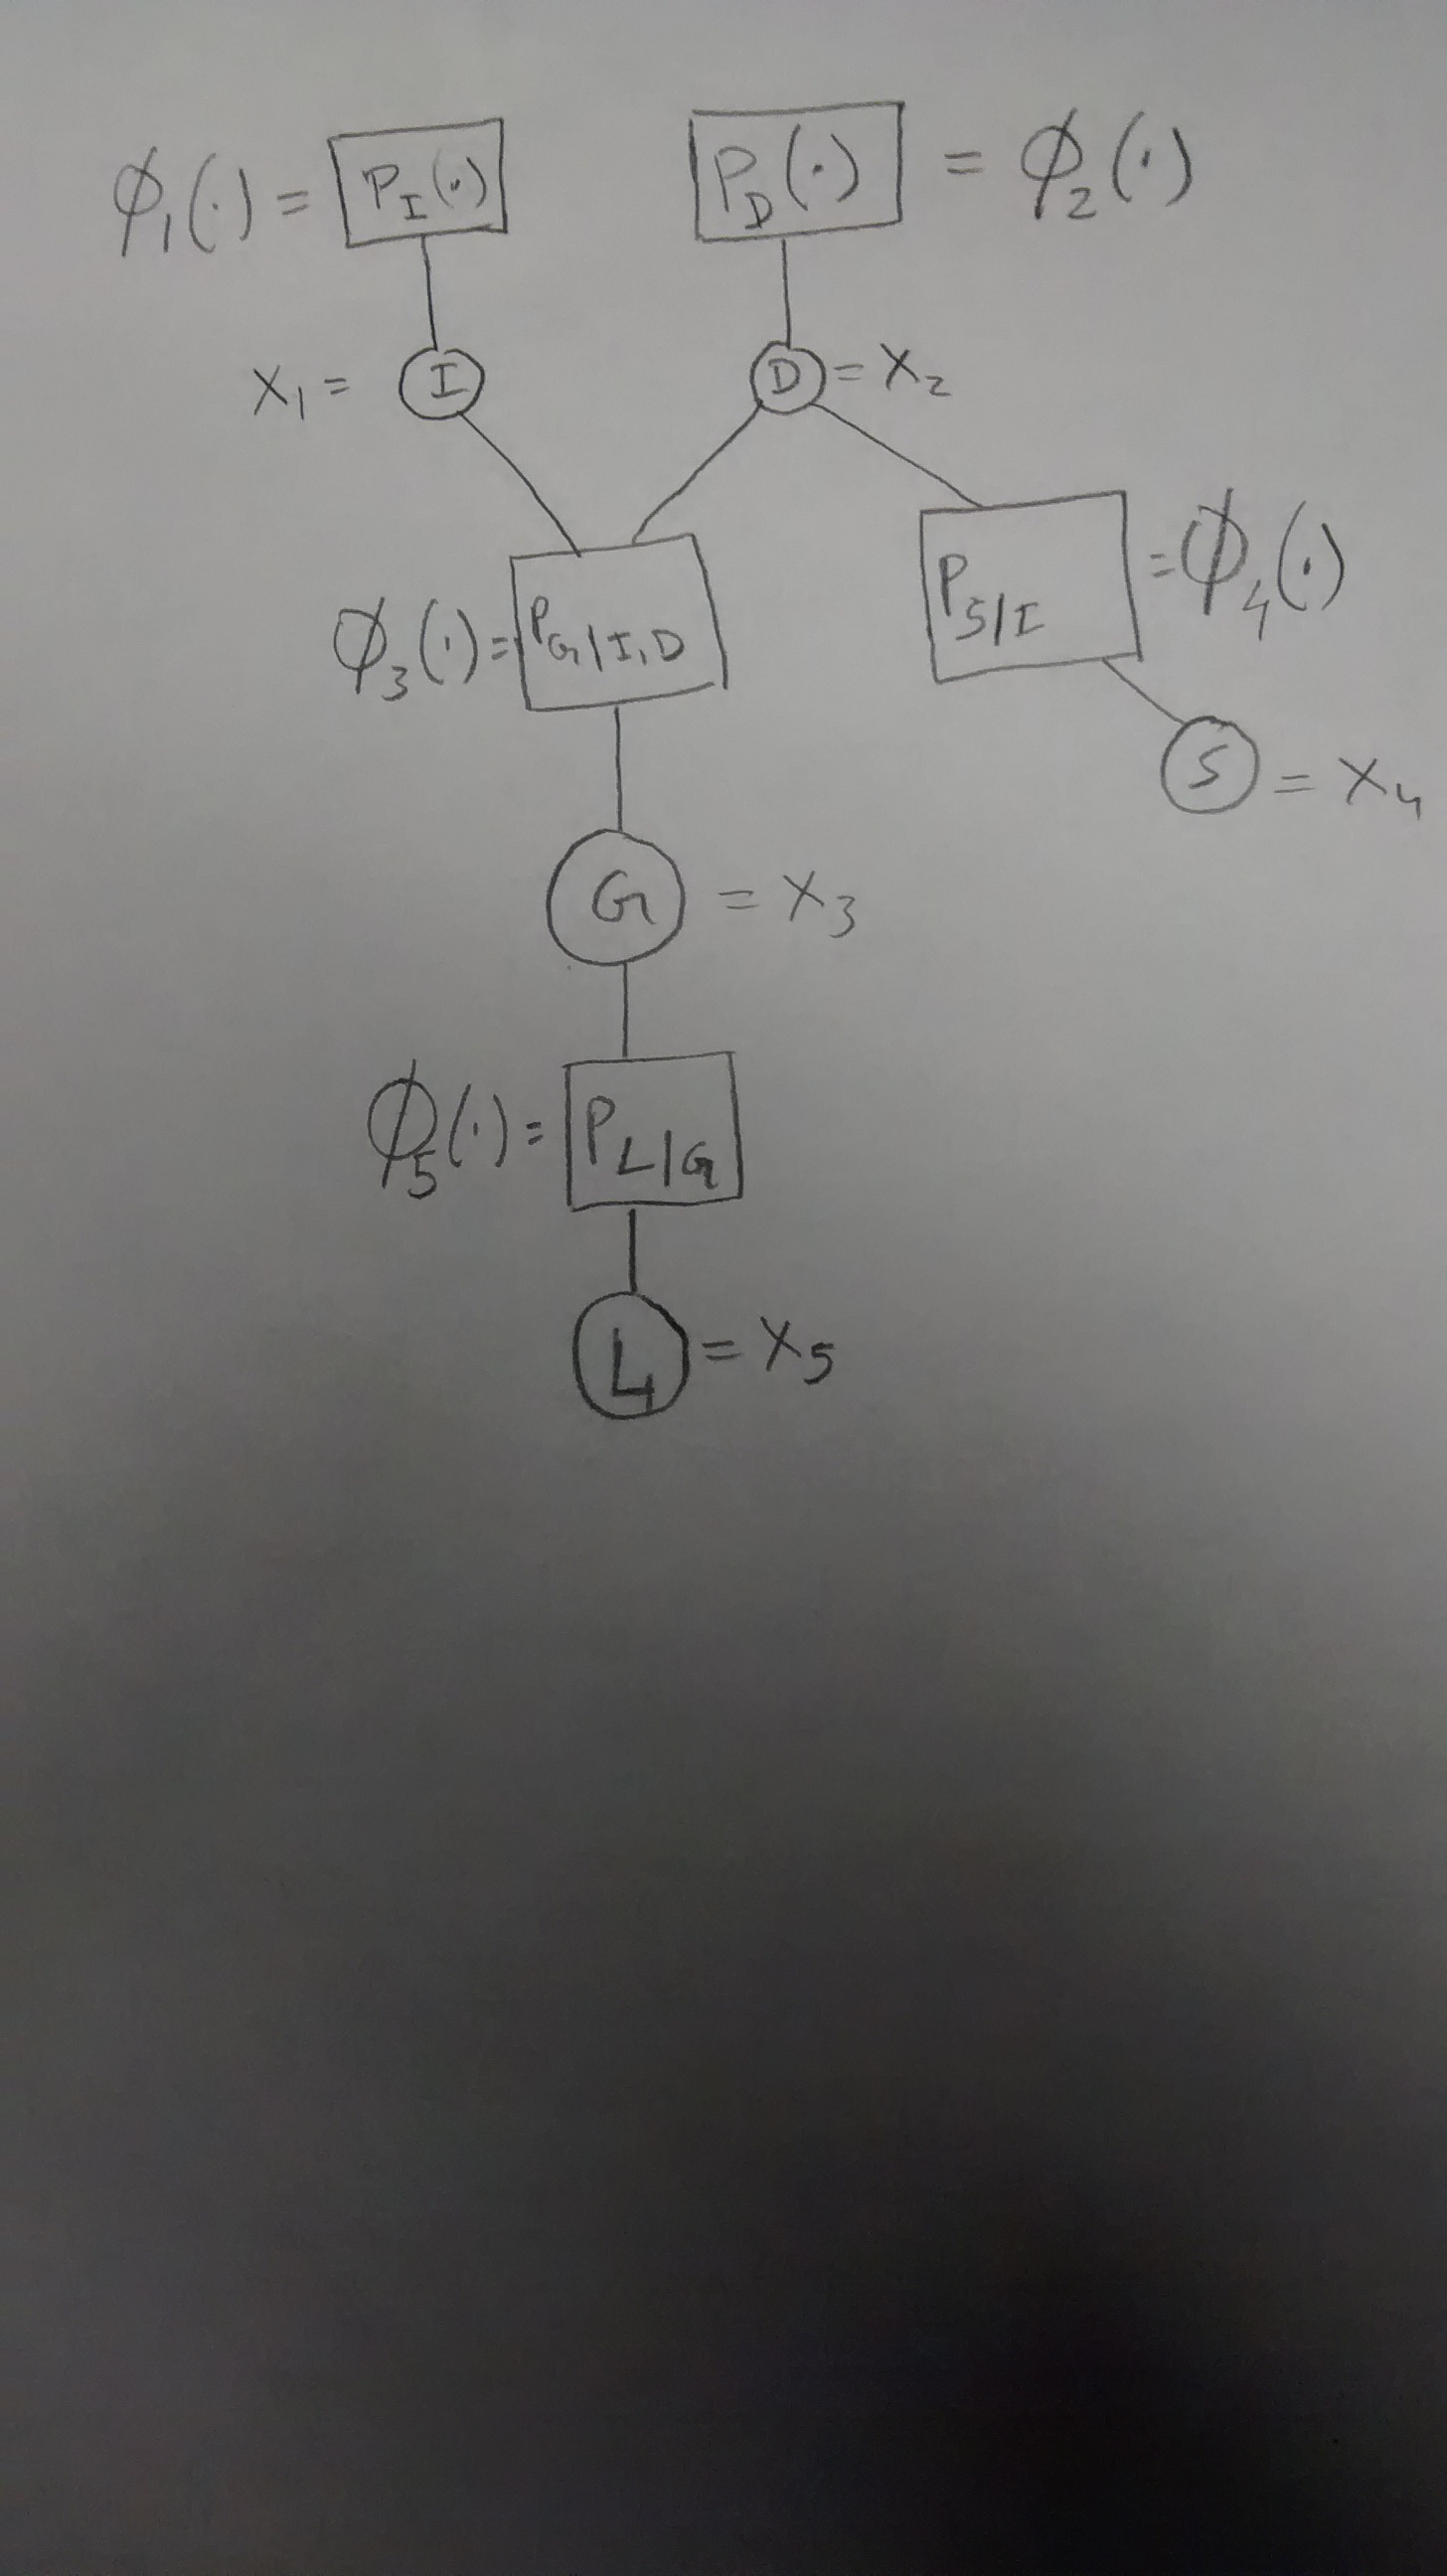
\includegraphics[height=0.58\textwidth, trim=0 15in 0 0, clip]{media/fg2.jpg}
  \caption{Factor graph representation with numbering}
  \label{fig:fg2}
\end{figure}

With this example, we are ready for a general definition of \emph{factor
graph}. 

A \emph{factor graph} is a three-tuple $(V, F, E)$ where $V$ is a set of random
variables, $F$ is a set of factors and $E$ is a set of undirected edges such
that $E = \{(X_i, \phi_j) | X_i \in V, \phi_j \in F, \phi_j \text{ depends on } X_i\}$.

\subsection{Coding the graphical model}


\subsection{Adapting the problem.}
Suppose we want to find out the probability of Letter being $l^1$ given SAT score is $s^0$. Mathematically, the 

\section{Generalization}

\end{document}
